%%%%%%%%%%%%%%
%% Run LaTeX on this file several times to get Table of Contents,
%% cross-references, and citations.

%% If you have font problems, you may edit the w-bookps.sty file
%% to customize the font names to match those on your system.

%% w-bksamp.tex. Current Version: Feb 16, 2012
%%%%%%%%%%%%%%%%%%%%%%%%%%%%%%%%%%%%%%%%%%%%%%%%%%%%%%%%%%%%%%%%
%
%  Sample file for
%  Wiley Book Style, Design No.: SD 001B, 7x10
%  Wiley Book Style, Design No.: SD 004B, 6x9
%
%
%  Prepared by Amy Hendrickson, TeXnology Inc.
%  http://www.texnology.com
%%%%%%%%%%%%%%%%%%%%%%%%%%%%%%%%%%%%%%%%%%%%%%%%%%%%%%%%%%%%%%%%

%%%%%%%%%%%%%
% 7x10
%\documentclass{wileySev}

% 6x9
\documentclass{wileySix}

\usepackage{graphicx}
\usepackage{listings}
\usepackage{float}
\usepackage[urlcolor=blue, colorlinks=true]{hyperref}
\usepackage{textcomp}
\usepackage{gensymb}
\usepackage{color}
 
\definecolor{codegreen}{rgb}{0,0.6,0}
\definecolor{codegray}{rgb}{0.5,0.5,0.5}
\definecolor{codepurple}{rgb}{0.58,0,0.82}
\definecolor{backcolour}{rgb}{0.95,0.95,0.92}
 
\lstdefinestyle{mystyle}{
    backgroundcolor=\color{backcolour},   
    commentstyle=\color{codegreen},
    keywordstyle=\color{magenta},
    numberstyle=\tiny\color{codegray},
    stringstyle=\color{codepurple},
    basicstyle=\footnotesize,
    breakatwhitespace=false,         
    breaklines=true,                 
    captionpos=b,                    
    keepspaces=true,                 
    numbers=left,                    
    numbersep=5pt,                  
    showspaces=false,                
    showstringspaces=false,
    showtabs=false,                  
    tabsize=2,
    language=sh
}
 
\lstset{style=mystyle}

%%%%%%%
%% for times math: However, this package disables bold math (!)
%% \mathbf{x} will still work, but you will not have bold math
%% in section heads or chapter titles. If you don't use math
%% in those environments, mathptmx might be a good choice.

% \usepackage{mathptmx}

% For PostScript text
\usepackage{w-bookps}

%%%%%%%%%%%%%%%%%%%%%%%%%%%%%%%%%%%%%%%%%%%%%%%%%%%%%%%%%%%%%%%%
%% Other packages you might want to use:

% for chapter bibliography made with BibTeX
% \usepackage{chapterbib}

% for multiple indices
% \usepackage{multind}

% for answers to problems
% \usepackage{answers}

%%%%%%%%%%%%%%%%%%%%%%%%%%%%%%
%% Change options here if you want:
%%
%% How many levels of section head would you like numbered?
%% 0= no section numbers, 1= section, 2= subsection, 3= subsubsection
%%==>>
\setcounter{secnumdepth}{3}

%% How many levels of section head would you like to appear in the
%% Table of Contents?
%% 0= chapter titles, 1= section titles, 2= subsection titles, 
%% 3= subsubsection titles.
%%==>>
\setcounter{tocdepth}{2}

%% Cropmarks? good for final page makeup
%% \docropmarks

%%%%%%%%%%%%%%%%%%%%%%%%%%%%%%
%
% DRAFT
%
% Uncomment to get double spacing between lines, current date and time
% printed at bottom of page.
% \draft
% (If you want to keep tables from becoming double spaced also uncomment
% this):
% \renewcommand{\arraystretch}{0.6}
%%%%%%%%%%%%%%%%%%%%%%%%%%%%%%

%%%%%%% Demo of section head containing sample macro:
%% To get a macro to expand correctly in a section head, with upper and
%% lower case math, put the definition and set the box 
%% before \begin{document}, so that when it appears in the 
%% table of contents it will also work:

\newcommand{\VT}[1]{\ensuremath{{V_{T#1}}}}

%% use a box to expand the macro before we put it into the section head:

\newbox\sectsavebox
\setbox\sectsavebox=\hbox{\boldmath\VT{xyz}}

%%%%%%%%%%%%%%%%% End Demo


\begin{document}


\booktitle{Cerdas Menguasai Git}
\subtitle{Dalam 24 Jam}

\authors{Rolly M. Awangga\\
\affil{Informatics Research Center}
%Floyd J. Fowler, Jr.\\
%\affil{University of New Mexico}
}

\offprintinfo{Cerdas Menguasai Git, First Edition}{Rolly M. Awangga}

%% Can use \\ if title, and edition are too wide, ie,
%% \offprintinfo{Survey Methodology,\\ Second Edition}{Robert M. Groves}

%%%%%%%%%%%%%%%%%%%%%%%%%%%%%%
%% 
\halftitlepage

\titlepage


\begin{copyrightpage}{2019}
%Survey Methodology / Robert M. Groves . . . [et al.].
%\       p. cm.---(Wiley series in survey methodology)
%\    ``Wiley-Interscience."
%\    Includes bibliographical references and index.
%\    ISBN 0-471-48348-6 (pbk.)
%\    1. Surveys---Methodology.  2. Social 
%\  sciences---Research---Statistical methods.  I. Groves, Robert M.  II. %
%Series.\\
%
%HA31.2.S873 2007
%001.4'33---dc22                                             2004044064
\end{copyrightpage}

\dedication{`Jika Kamu tidak dapat menahan lelahnya belajar, 
Maka kamu harus sanggup menahan perihnya Kebodohan.'
~Imam Syafi'i~}

\begin{contributors}
\name{Rolly Maulana Awangga,} Informatics Research Center., Politeknik Pos Indonesia, Bandung,
Indonesia



\end{contributors}

\contentsinbrief
\tableofcontents
%\listoffigures
%\listoftables
%\lstlistoflistings


\begin{foreword}
Sepatah kata dari Kaprodi, Kabag Kemahasiswaan dan Mahasiswa
\end{foreword}

\begin{preface}
Buku ini diciptakan bagi yang awam dengan git sekalipun.

\prefaceauthor{R. M. Awangga}
\where{Bandung, Jawa Barat\\
Februari, 2019}
\end{preface}


\begin{acknowledgments}
Terima kasih atas semua masukan dari para mahasiswa agar bisa membuat buku ini 
lebih baik dan lebih mudah dimengerti.

Terima kasih ini juga ditujukan khusus untuk team IRC yang 
telah fokus untuk belajar dan memahami bagaimana buku ini mendampingi proses 
Intership.
\authorinitials{R. M. A.}
\end{acknowledgments}

\begin{acronyms}
\acro{ACGIH}{American Conference of Governmental Industrial Hygienists}
\acro{AEC}{Atomic Energy Commission}
\acro{OSHA}{Occupational Health and Safety Commission}
\acro{SAMA}{Scientific Apparatus Makers Association}
\end{acronyms}

\begin{glossary}
\term{git}Merupakan manajemen sumber kode yang dibuat oleh linus torvald.

\term{bash}Merupakan bahasa sistem operasi berbasiskan *NIX.

\term{linux}Sistem operasi berbasis sumber kode terbuka yang dibuat oleh Linus Torvald
\end{glossary}

\begin{symbols}
\term{A}Amplitude

\term{\hbox{\&}}Propositional logic symbol 

\term{a}Filter Coefficient

\bigskip

\term{\mathcal{B}}Number of Beats
\end{symbols}


%%%%%%%%%%%%%%%%%%Isi Buku_

\chapter{Chapter 1}
%\section{Dinda Anik Masruro - 1184003}
\subsection{Teori}
\begin{enumerate}

	\item Definisi Kecerdasan Buatan
	\hfill\break
	Kecerdasan Buatan atau biasa disebut dengan istilah AI (Artificial Intelligence). Kecerdasan Buatan adalah salah satu bidang studi yang berhubungan dengan pemanfaatan mesin untuk memecahkan persoalan yang rumit dengan cara lebih manusiawi dan lebih bisa di pahami oleh manusia. Kecerdasan buatan makin canggih dengan kemampuan komputer dalam memperbarui pengetahuannya dengan banyaknya testing dan perkembangan target analisa. Untuk kecerdasan buatan ada banyak contoh dan jenisnya. Salah satu contoh yang paling terkenal dari Artificial Intelligence ialah Google Assistant. Google Assistant digunakan untuk kemudahan user dalam menemukan berbagai hal maupun penyetingan langsung terhadap smartphone yang digunakan dan masih banyak lagi.

	\item Sejarah dan Perkembangan
	\hfill\break
    Pada tahun 1943, pekerjaan pertama yang dikenal sebagai AI atau \textit{Artificial Intellegent} telah dikemukakan oleh Warren McCulloch dan juga Walter Pits yang dinamakan sebagai artificial neurons. Kemudian pada tahun 1955, Allen Newell dan Herbert A. Simon membuat program kecerdasan buatan pertama yang dinamakan Logic Theorist. Lalu pada tahun 1972, robot pertama dibuat di jepang dengan nama Wabot-1 dengan kecerdasan buatan. Pada tahun 1980, muncul bidang baru dari kecerdasan buatan yaitu Expert System yang membantu dalam pemberian keputusan. Kemudian pada tahun 1997, IBM deep blue mengalahkan juara catur dunia Gary Kasparov dan menjadi komputer pertama yang mengalahkannya. Tahub 2006, perusahaaan sudah mulai menerapkan kecerdasan buatan pada produknya seperti Netflix dan Twitter. Tahun 2018, Project Debater dari IBM melakuakn debat tentang topik yang kompleks dan berakhir dengan hasil memuaskan.
	
	\item Kecerdasan buatan terbagi atas beberapa metode yaitu:
	\hfill\break
	Supervised learning,  Klasifikasi, Regresi,Unsupervised Learning, Dataset, Trainingset dan juga Testingset.
	\begin{itemize}
		\item Supervised Learning
		\hfill\break
	Supervised Learning adalah sebuah tipe learning yang mempunyai variable input dan variable output, tipe ini juga menggunakan satu algoritma atau lebih dari satu algoritma yang digunakan untuk mempelajari fungsi  pemetaan dari input ke output.
		\item Klasifikasi
		\hfill\break
		Klasifikasi merupakan suatu kegiatan dari penggolongan atau pengelompokkan. Tetapi secara umum klasifikasi merupakan suatu kegiatan yang dapat mengelompokkan benda-benda yang memiliki beberapa ciri-ciri yang sama dan memisahkan benda yang tidak sama. 
		\item Regresi
		\hfill\break
        Regresi adalah metode analisis statistik yang digunakan untuk dapat melihat efek antara dua atau lebih variabel. Hubungan variabel dalam pertanyaan adalah fungsional yang diwujudkan dalam bentuk model matematika. Dalam analisis regresi, variabel dibagi menjadi dua jenis, yaitu variabel respons atau yang biasa disebut variabel dependen dan variabel independen atau dikenal sebagai variabel independen. Ada beberapa jenis analisis regresi, yaitu regresi sederhana yang mencakup linear sederhana dan regresi non-linear sederhana dan regresi berganda yang mencakup banyak linier atau non-linear berganda. Analisis regresi digunakan dalam pembelajaran mesin pembelajaran dengan metode pembelajaran terawasi.
		\item Unsupervised Learning 
		\hfill\break
        Unsupervised Learning merupakan pelatihan algoritma kecerdasan buatan (AI) menggunakan informasi yang tidak diklasifikasikan atau diberi label dan memungkinkan algoritma untuk bertindak atas informasi tersebut tanpa bimbingan. Dalam Unsupervised Learning, sistem AI dapat mengelompokkan informasi yang tidak disortir berdasarkan persamaan dan perbedaan meskipun tidak ada kategori yang disediakan.
		\item Data set
		\hfill\break
        Data set adalah objek yang merepresentasikan data dan relasinya di memory. Strukturnya mirip dengan data di database. Dataset berisi koleksi dari datatable dan datarelation.
		\item Training Set
		\hfill\break
    	Training set merupakan bagian dari data set yang di latih untuk membuat prediksi atau menjalankan fungsi dari algoritma ML lain sesuai dengan masing-masing. Memberikan instruksi melalui algoritma sehingga mesin yang di praktikkan dapat menemukan korelasinya sendiri.	
		\item Testing Set
		\hfill\break
        Testing set adalah bagian dari data set yang di uji untuk melihat akurasinya, atau dengan kata lain untuk melihat kinerjanya.
	\end{itemize}
\end{enumerate}
\subsection{Praktek}
\begin{enumerate}
	\item Instalasi Library scikit dari Anaconda, mencoba kompilasi dan uji coba ambil contoh kode dan lihat variabel explorer
	\hfill\break
	\begin{figure}[h]
		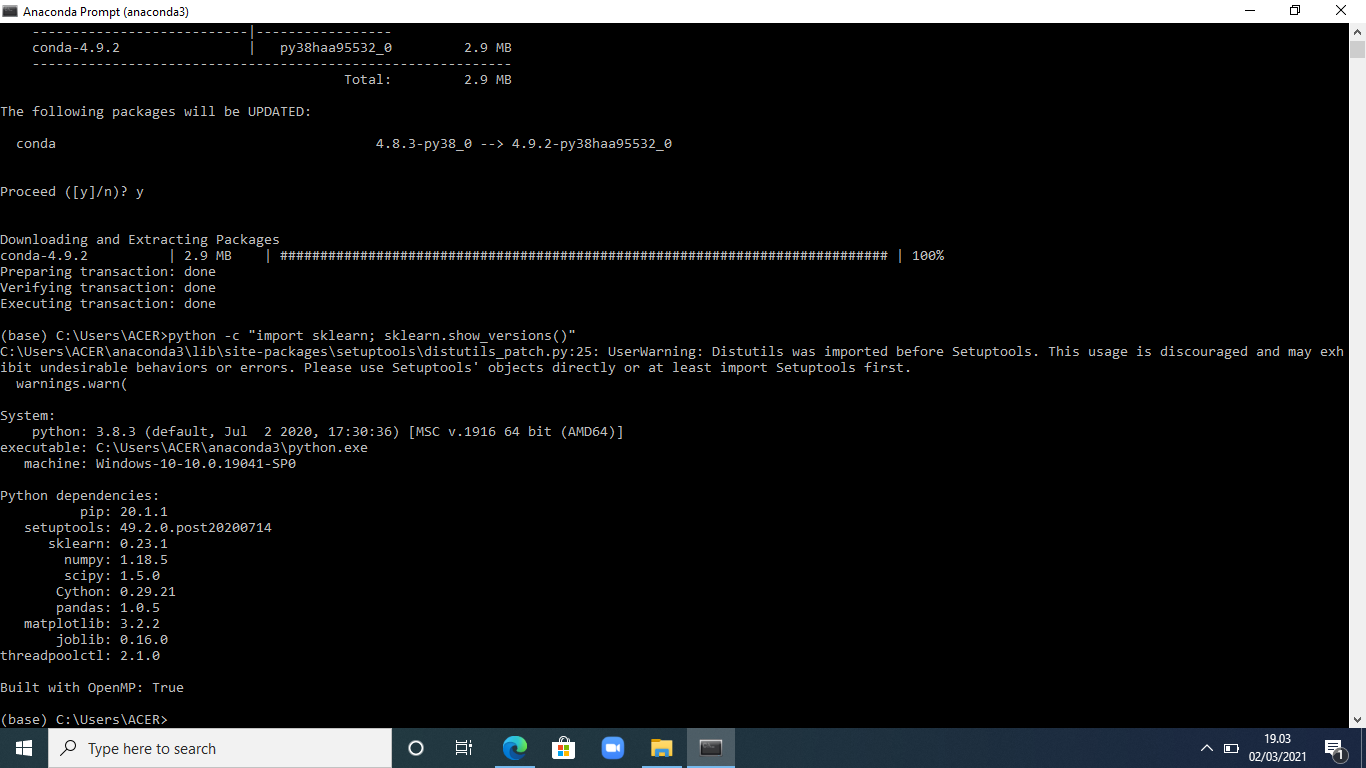
\includegraphics[width=10cm]{figures/1184003/chapter1/1.png}
		\centering
		\caption{Instalasi Library Scikit Learn}
	\end{figure}
	\begin{figure}[h]
		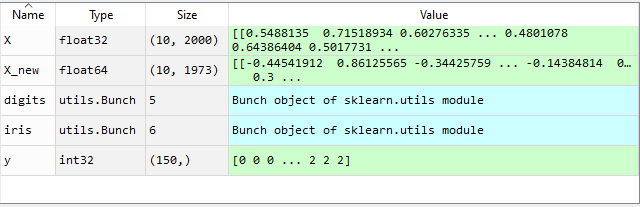
\includegraphics[width=10cm]{figures/1184003/chapter1/2.PNG}
		\centering
		\caption{Isi Variabel Explorer}
	\end{figure}
	\newpage\item Uji coba loading an example dataset
	\hfill\break
\lstinputlisting[firstline=7, lastline=16]{src/tugas1.py}
\item Uji coba Learning dan predicting
	\hfill\break
	\lstinputlisting[firstline=17, lastline=32]{src/tugas1.py}
\item Uji coba Model Persistence
	\hfill\break
	\lstinputlisting[firstline=35, lastline=63]{src/tugas1.py}	
	\item Uji coba Conventions
	\hfill\break
	\lstinputlisting[firstline=64, lastline=82]{src/tugas1.py}
	\end{enumerate}
	\subsection{Penanganan Error}
\begin{enumerate}
	\item ScreenShoot Error
	\begin{figure}[h]
		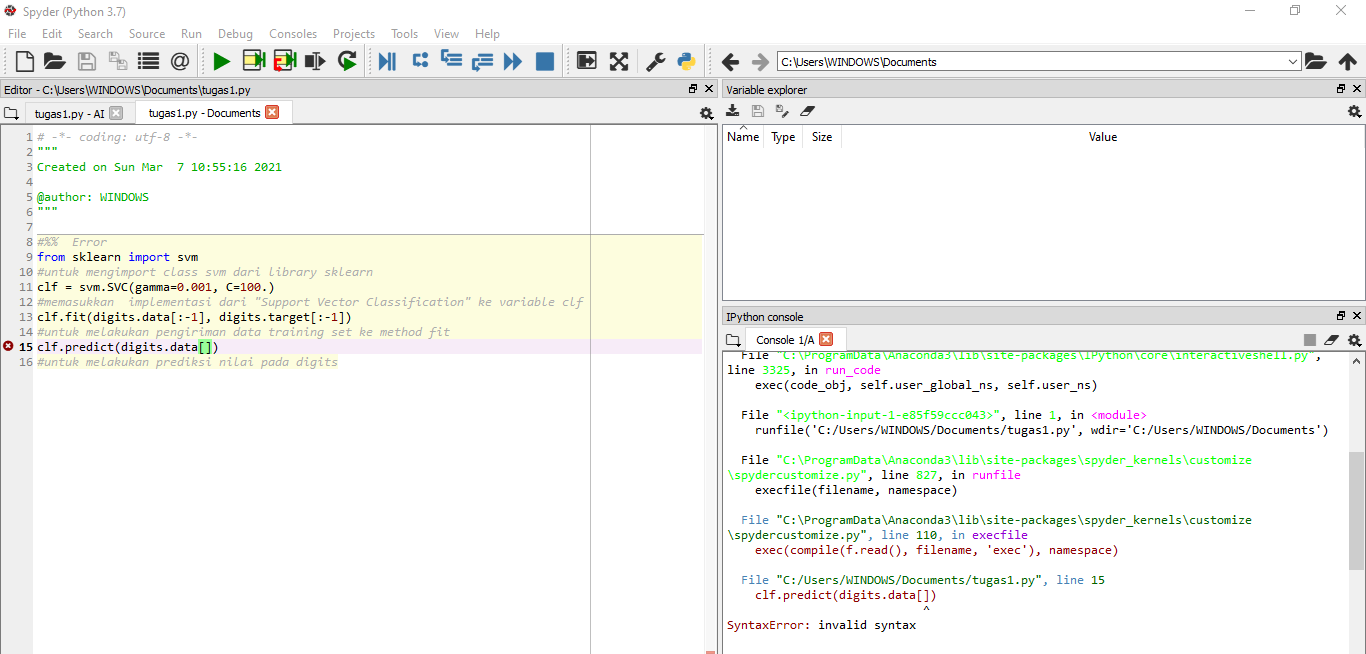
\includegraphics[width=10cm]{figures/1184003/chapter1/3.PNG}
		\centering
		\caption{Name Error}
	\end{figure}
	\newpage\item Tuliskan Kode Error dan Jenis Error
	\hfill\break
	\lstinputlisting[firstline=83, lastline=91]{src/tugas1.py}
\hfill\break
	\item Cara Penangan Error
\hfill\break Tambahkan prediksi nilainya agar kode program dapat terbaca
	\end{enumerate}
	\subsection{Bukti Tidak Plagiat}
\begin{figure}[h]
	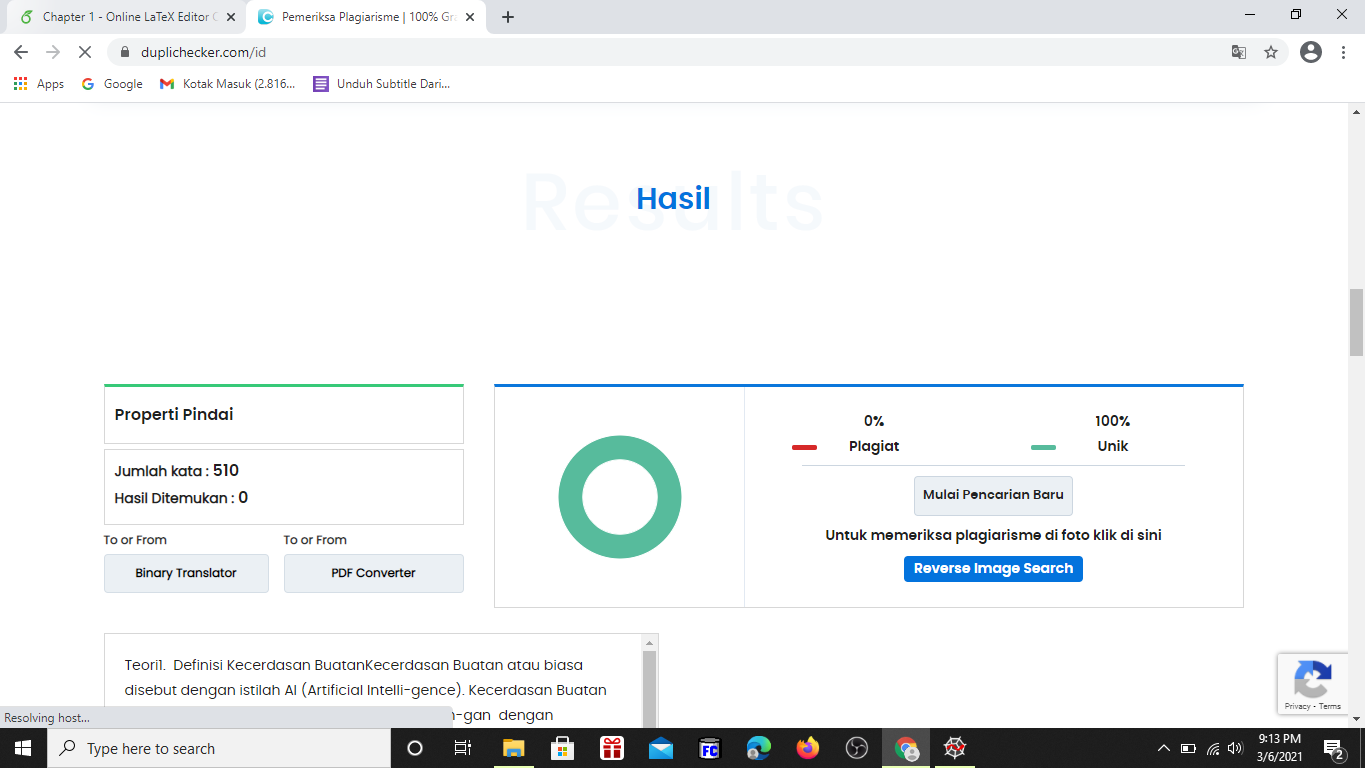
\includegraphics[width=10cm]{figures/1184003/chapter1/4.png}
	\centering
	\caption{Bukti Tidak Melakukan Plagiat Chapter 1}
\end{figure}
%\section{1184006 - Murnia Lestari}
\subsection{Teori}
\begin{enumerate}

	\item Definisi Kecerdasan Buatan
	\hfill\break
	Kecerdasan Buatan atau Artifical Inteligence yang terdiri dari kata cerdas dan buatan. Cerdas artiya cepat dan tepat.  Sedangkan buatan artinya sesuatu yang sengaja dibuat dengan tujuan tertentu. Jadi kecerdasan buatan merupakan sebuah sistem yang disimulasikan dari kecerdasan yang dipunyai oleh manusia. Sehingga sistem ini akan melakukan pelkerjaan-pekerjaan yang umumnya dikerjakan oleh manusia secara cepat dan tepat seperti yang dilakukan oleh manusia. Point-point penting yang terdapat  dalam proses kecerdasan buatan adalah learning,reasoning dan self correction.

	\item Sejarah dan Perkembangan
	\hfill\break
Kecerdasan buatan bermula pada tahun 1940-an yang bermula dari kemunculan komputer. Kemudia pada tahun 1943 McMulloh dan Pitts pada tahun 1943 mempunyai usul untuk membuat model matematis yang bernama percepton dari neurin yang ada didalam otak. Pada tahun 1950 terbuatlah mesin turing yang mencoba menjawab “dapatkah computer berpikir” yang terdapat pada paper Alan Turing. Pada tahun 1955 akhir,Newell dan simon mengembangkan The Logic Theorist yaitu program kecerdasan buatan yang pertama. Pada tahun 1956 dari Massacuhetts Institute of Technology yaitu John McCharty yang dianggap sebagai bapak dari kecerdasan buatan atau AI menyelenggarakan konferensi untuk para ahli komputer dengan nama “ The Dartmouth summer research project on artifical intelligence. Pada tahun 1960-1970 muncullah “classical AI” yang merupakan diskusi mengenai bagaimana komputer dapat meniru dengan detail kemmapuan otak manusia. Dan pada tahun 1980 merupakan titik dimna kecerdasan buatan berkembang karena komputer dapat diperoleh dengan harga yag lebih murah.
	

	\item Kecerdasan buatan terbagi atas beberapa metode yaitu:
	\hfill\break
	Supervised learning,  Klasifikasi, Regresi,Unsupervised Learning, Dataset, Trainingset dan juga Testingset.
	\begin{itemize}
		\item Supervised Learning
		\hfill\break
	Supervised Learning	merupakan algoritma yang memiliki attribut tambahan seperti x dan y yang ingin diprediksi.
		\item Klasifikasi
		\hfill\break
		Klasifikasi merupakan sampel yang dimiliki oleh dua atau lebih kelas yang dikelompokkan yang disesuaikan berdasarkan ukuran kemiripan atau jarak yang melekat. 
		\item Regresi
		\hfill\break
Regresi	merupakan sebuah prediksi apabila hasil atau output yang diinginkan terdiri dari satu atau lebih variable contionous.
		\item Unsupervised Learning 
		\hfill\break
Unsupervised Learning  merupakan	algoritma yang tidak memiliki attribut tambahan yang akan diprediksi
		\item Data set
		\hfill\break
Data set	merupakan kondisi dimana hanya terdapat inputan data tanpa memiliki viariasi output yang sesuai
		\item Training Set
		\hfill\break
	Training Set	merupakan bagian dari data set yang digunakan untuk mempelajari beberapa properti		
		\item Testing Set
		\hfill\break
Testing Set	merupakan bagian data set yang digunakan untuk pengujian dari properti yang dipelajari
	\end{itemize}
\end{enumerate}
\subsection{Praktek}
\begin{enumerate}
	\item Instalasi Library scikit dari Anaconda, mencoba kompilasi dan uji coba ambil contoh kode dan lihat variabel explorer
	\hfill\break
	\begin{figure}[h]
		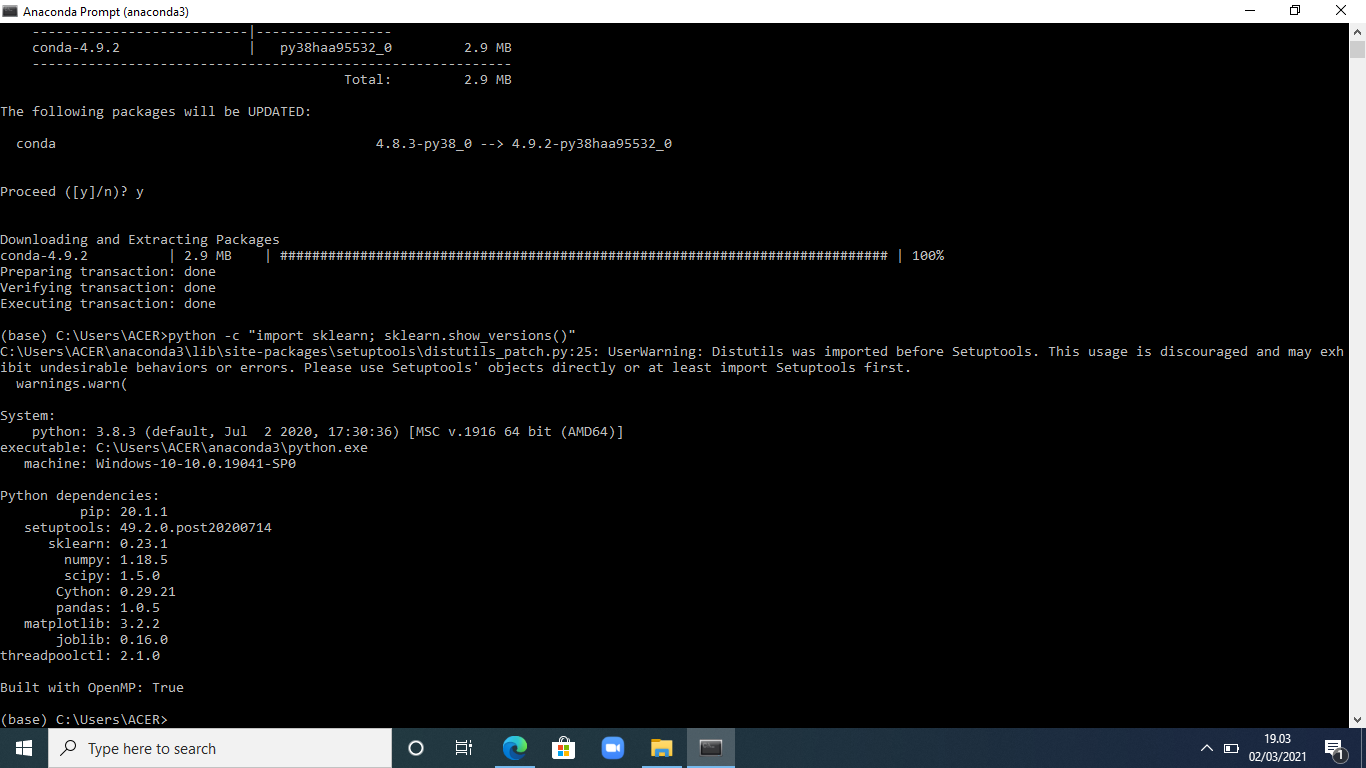
\includegraphics[width=10cm]{figures/1184006/chapter1/01.png}
		\centering
		\caption{Instalasi Library Scikit Learn}
	\end{figure}
	\begin{figure}[h]
		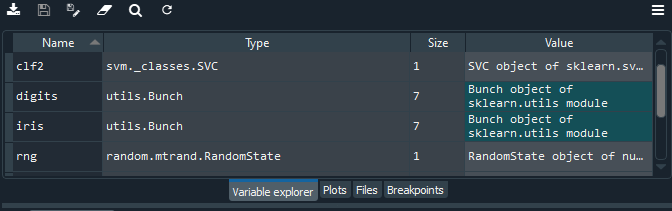
\includegraphics[width=10cm]{figures/1184006/chapter1/02.PNG}
		\centering
		\caption{Isi Variabel Explorer}
	\end{figure}
	\newpage\item Uji coba loading an example dataset
	\hfill\break
\lstinputlisting[firstline=7, lastline=16]{src/1184006/chapter1/tugas1.py}
\item Uji coba Learning dan predicting
	\hfill\break
	\lstinputlisting[firstline=17, lastline=32]{src/1184006/chapter1/tugas1.py}
\item Uji coba Model Persistence
	\hfill\break
	\lstinputlisting[firstline=35, lastline=63]{src/1184006/chapter1/tugas1.py}
	\item Uji coba Conventions
	\hfill\break
	\lstinputlisting[firstline=64, lastline=82]{src/1184006/chapter1/tugas1.py}
	\end{enumerate}
	\subsection{Penanganan Error}
\begin{enumerate}
	\item ScreenShoot Error
	\begin{figure}[h]
		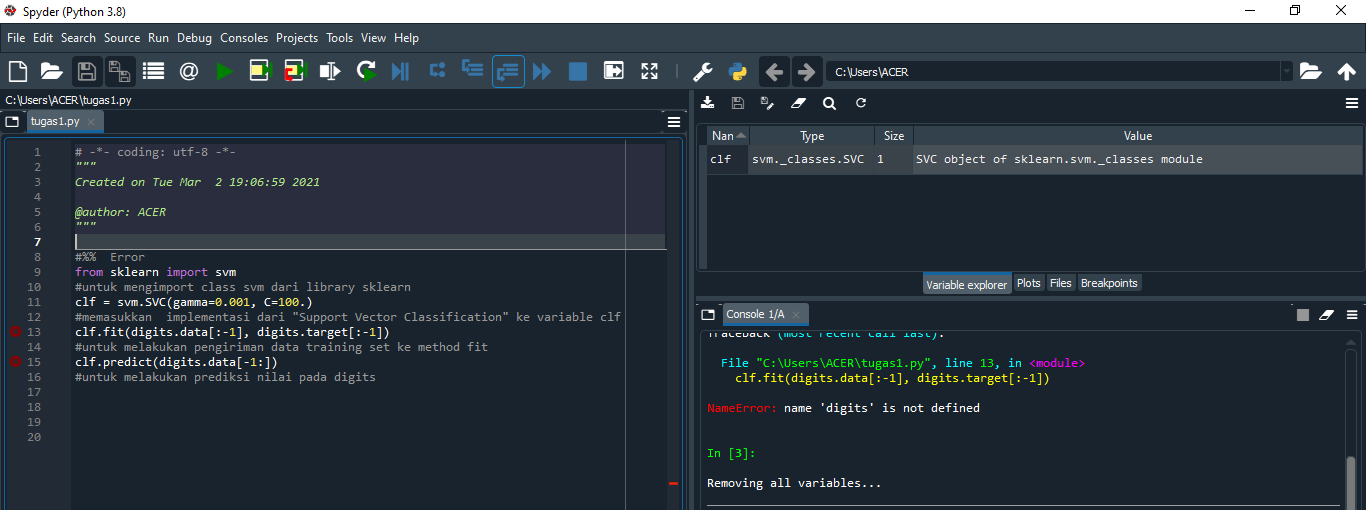
\includegraphics[width=10cm]{figures/1184006/chapter1/03.PNG}
		\centering
		\caption{Name Error}
	\end{figure}
	\newpage\item Tuliskan Kode Error dan Jenis Error
	\hfill\break
	\lstinputlisting[firstline=83, lastline=91]{src/1184006/chapter1/tugas1.py}
\hfill\break
	\item Cara Penangan Error
\hfill\break Tambahkan variabel digits agar kode program dapat terbaca
	\end{enumerate}
	\subsection{Bukti Tidak Plagiat}
\begin{figure}[h]
	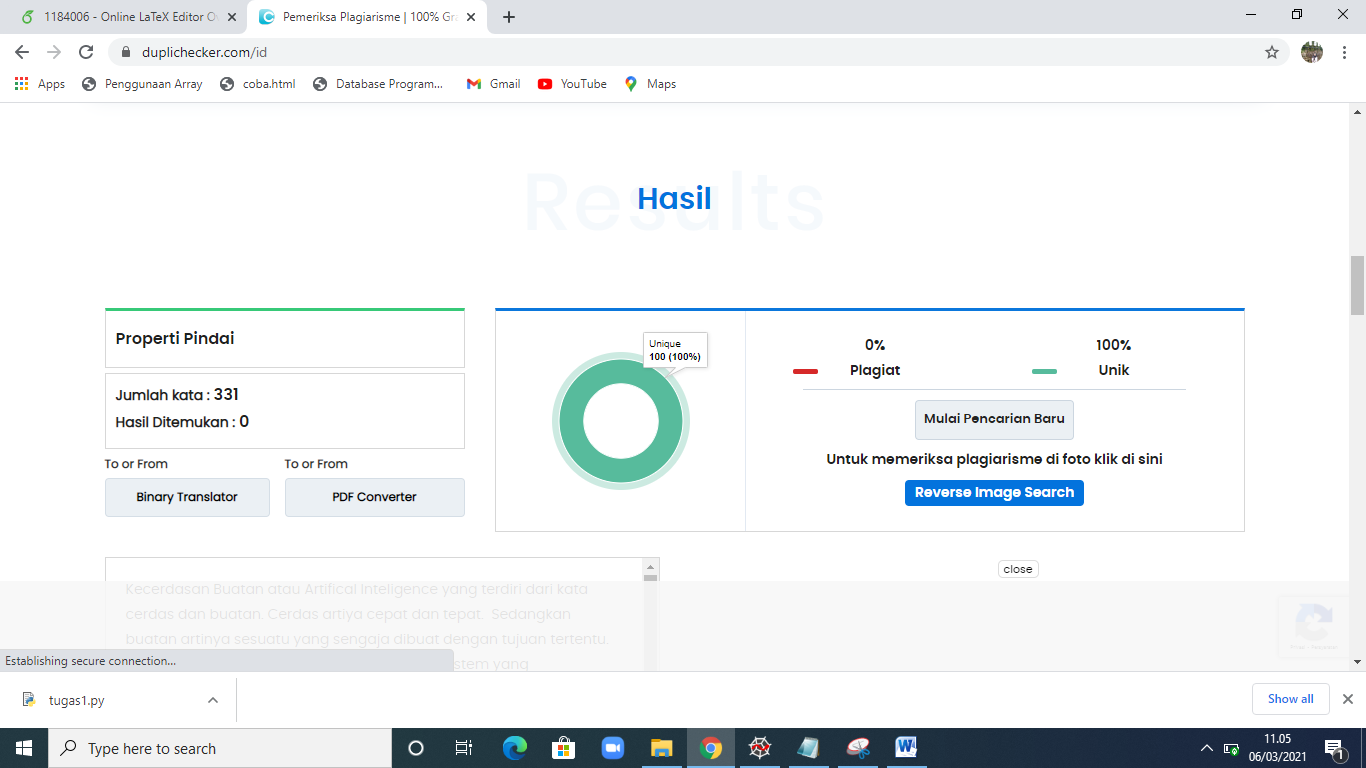
\includegraphics[width=10cm]{figures/1184006/chapter1/04.png}
	\centering
	\caption{Bukti Tidak Melakukan Plagiat Chapter 1}
\end{figure}
%\section{1184071 - Annisa Khairani Febrianti}
\subsection{Teori}
\begin{enumerate}
	\item Definisi Kecerdasan Buatan (AI)
	\hfill\break
	Kecerdasan Buatan atau \textit{Artificial Intelligence} (AI) merupakan teknik meniru kecerdasan yang dimiliki oleh makhluk hidup maupun benda mati untuk menyelesaikan suatu masalah. Atau dapat di definisikan sebagai salah satu cabang Ilmu pengetahuan yang berkaitan dengan pemanfaatan mesin untuk menyelesaikan persoalan rumit dengan menggunakan cara yang lebih manusiawi. Adapun contoh sederhana penerapan kecerdasan buatan adalah SIRI, bagi pengguna iphone atau \textit{IOS} pasti sudah tidak asing dengan SIRI yang
    seringkali diartikan sebagai asisten pribadi pengguna IOS dalam melakukan hal-hal tertentu untuk penggunanya.

	\item Perkembangan dan Sejarah AI
	\hfill\break
	Pada tahun 1956 merupakan tahun pertama kali muncul istilah AI atau \textit{Artificial Intellegent} yang dikemukakan oleh \textbf{John McCarthy} di Konferensi Darthmouth.Penggunaan AI begitu popular dari tahun ke tahun. Pada tahun 1950-an merupakan tahap dimana riset awal proyek AI yang tujuan untuk eksplorasi topik penyelesaian persoalan dan metode simbolik.Selanjutnya Pada tahun 1959, Dari IBM yang bernama \textbf{Nathaniel Rochester} bersama beberapa mahasiswa lainnya mengeluarkan program kecerdasan buatan yaitu \textit{Geometry Theorm Prover}. Lalu pada tahun 1960-an Departemen Pertahanan yang berasal dari Amerika Serikat memiliki keinginan dalam melatih dan mengembangkan komputer supaya memiliki nalar yang menyerupai manusia secara dasar. Kemudian Pada tahun 1963, program yang mampu menyelesaikan masalah integral tertutup untuk mata kuliah Kalkulus dibuat dengan \textbf{James Slagle}. Pada tahun 1970-an, adanya suatu keberhasilan proyek DARPA \textit{(Defence Advanced Research Project Agency)} dengan mampu menyelesaikan studi kasus tentang pemetaan jalan. Selanjutnya Pada tahun 1986, program analogi yang digunakan dalam pemecahan masalah analogi geometris yang ada pada tes IQ dibuatan oleh \textbf{Tom Evan}. Dari tahun 1980an AI kemudian mulai berkembang dibidang idustri dan mulai berkiprah hingga saat ini dimana para ilmuan berlomba-lomba untuk menciptakan AI yang bermanfaat pada kehidupan sekarang atau dimasa depan nanti. Setelah itu pada awal abad ke 21 atau lebih tepatnya pada tahun 2003, DARPA berhasil untuk menciptakan asisten pribadi yang cerdas. Sejak saat itu lah teknologi AI terus berkembang sangat bagus dan sampai saat ini AI tersebutlebih menjurus pada program yang lebih detail dan kompleks dengan penerapan struktur algoritma dari pembelajaran secara mendalam atau \textit{deep learning} yaitu AI yang dikembangkan bisa mengerjakan persoalan dan memberi solusi yang lebih kompleks dengan kondisi yang lebih beragam.

	\item Kecerdasan buatan (AI) terbagi menjadi beberapa metode yaitu:
	\hfill\break
	Supervised learning,  Klasifikasi, Regresi,Unsupervised Learning, Dataset, Trainingset dan juga Testingset.
	\begin{itemize}
		\item Supervised Learning
		\hfill\break
	Supervised learning merupakan suatu pembelajaran dengan adanya pengawas atau bisa disebut dengan supervisor. Supervisor merupakan suatu label yang ada di setiap data nya. Kemudian label tersebut berisi tag dari data yang ditambah ke dalam model pembelajaran mesin atau lebih trend disebut dengan \textbf{machine learning model}. Bisa diilustrasikan seperti gambar apel di tag “apel” dari masing-masing gambar tersebut apel dan gambar pir di tag “pir”dari masing-masing gambar pir. Lalu Machine learning memiliki berapa kategori berupa clasification (“apel”, “pir”, dsb) dan regression ( tinggi badan, berat badan, dsb).
		\item Klasifikasi
		\hfill\break
		Klasifikasi merupakan sampel yang dimiliki oleh dua atau lebih kelas yang dikelompokkan yang disesuaikan berdasarkan ukuran kemiripan atau jarak yang melekat. 
		\item Regresi
		\hfill\break
    Regresi	merupakan sebuah prediksi apabila hasil atau output yang diinginkan terdiri dari satu atau lebih variable contionous.
		\item Unsupervised Learning 
		\hfill\break
Unsupervised learning merupakan suatu pembelajaran tanpa adanya sebuah pengawasan dan tidak menggunakan label untuk bisa memprediksi target variable. Unsupervised learning lebih mengelompokan tentang kesamaan ataupun kemiripan dari attribut yang sudah diinputkan. Apabila attribut dan sifat dari data variable yang diproses ternyata memiliki kemiripan, maka akan dijadikan
satu kelompok (clustering). Dan akan menimbulkan beberapa bagian kelompok (cluster). Jumlah cluster bisa tidak terbatas. Dari kelompok tersebut model melabelkan, dan jika data baru akan di prediksi, itu akan diproses untuk mencocokan kelompok yang memiliki kemiripan feature. unsupervised learning tidak punya outcome spesifik seperti supervise learning karena tidak adanya sebuah label dasar.
\hfill\break
\textbf{Dapat disimpulkan Jika Supervised learning tentang atribut atau label yang sudah ada dari kategori yang diinginkan berbeda dengan unservised learning dimana unsupervised menggunakan kesamaan dari attribut yang dimiliki. Jika attribut dan sifat dari data feature yang diekstrak memiliki
kemiripan, maka akan dikelompokan kedalam \textit{(clustering)}. Sehingga hal ini
akan menimbulkan kelompok \textit{(cluster)}. Jumlah cluster bisa unlimited atau tidak terbatas}.
		\item Data Set
		\hfill\break
Data Set merupakan kumpulan sampel yang sudah dikumpulkan dan bersifat
homogen. Salah satu contohnya yaitu Seorang anak ingin bermain Voli, tetapi keputusannya untuk bermain voli tersebut tergantung pada variable yang ditentukan contohnya jarak kaki dari garis, atau tinggi net sehingga variable ini disebut dengan fitur dalam sebuah permainan.
		\item Training Set
		\hfill\break
Data yang digunakan untuk bisa melakukan klasifikasi ataupun prediksi,Dengan adanya data training maka akan didapatkan sebuah model regresi.		
		\item Testing Set
		\hfill\break
Testing Set digunakan untuk menguji kebenaran dari sebuah model data.Adapun Testing data berisi \textit{unseen example} merupakan contoh yang tidak ada didalam training set.
	\end{itemize}
\end{enumerate}
\subsection{Praktek}
\begin{enumerate}
	\item Instalasi Library scikit dari Anaconda, mencoba kompilasi dan uji coba ambil contoh kode dan lihat variabel explorer
	\hfill\break
	\begin{figure}[h]
		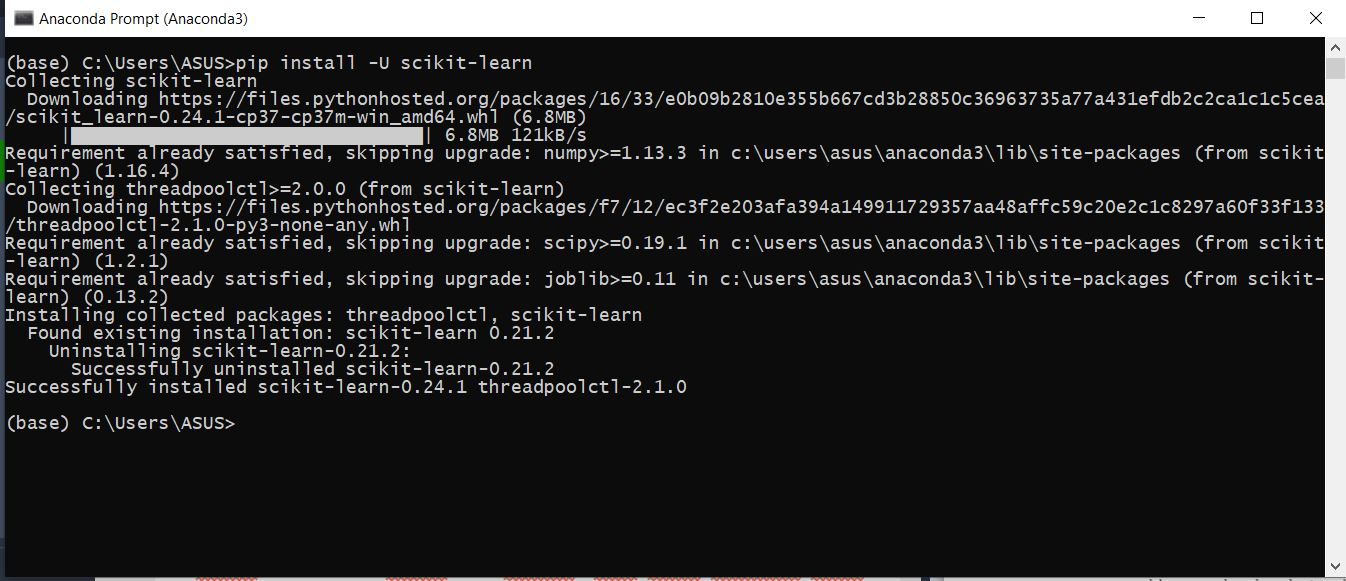
\includegraphics[width=12cm]{figures/1184071/chapter1/1.JPG}
		\centering
		\caption{Instalasi Library Scikit Learn}
	\end{figure}
	\begin{figure}[h]
		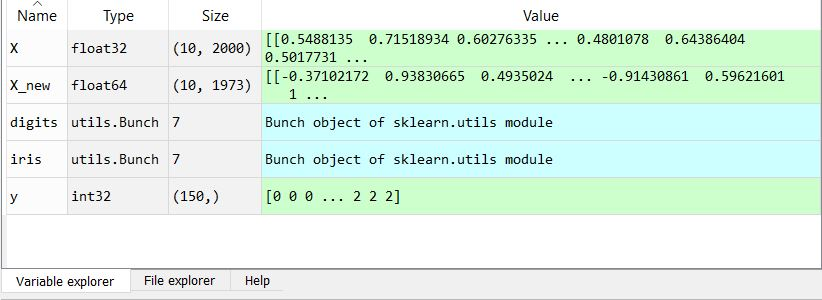
\includegraphics[width=15cm]{figures/1184071/chapter1/2.JPG}
		\centering
		\caption{Isi Variabel Explorer}
	\end{figure}
	\newpage\item Uji coba loading an example dataset
	\hfill\break
\lstinputlisting[firstline=7, lastline=16]{src/tugas1.py}
\item Uji coba Learning dan predicting
	\hfill\break
	\lstinputlisting[firstline=17, lastline=32]{src/tugas1.py}
\item Uji coba Model Persistence
	\hfill\break
	\lstinputlisting[firstline=35, lastline=63]{src/tugas1.py}	
	\item Uji coba Conventions
	\hfill\break
	\lstinputlisting[firstline=64, lastline=82]{src/tugas1.py}
	\end{enumerate}
	\subsection{Penanganan Error}
\begin{enumerate}
	\item ScreenShoot Error
	\begin{figure}[h]
		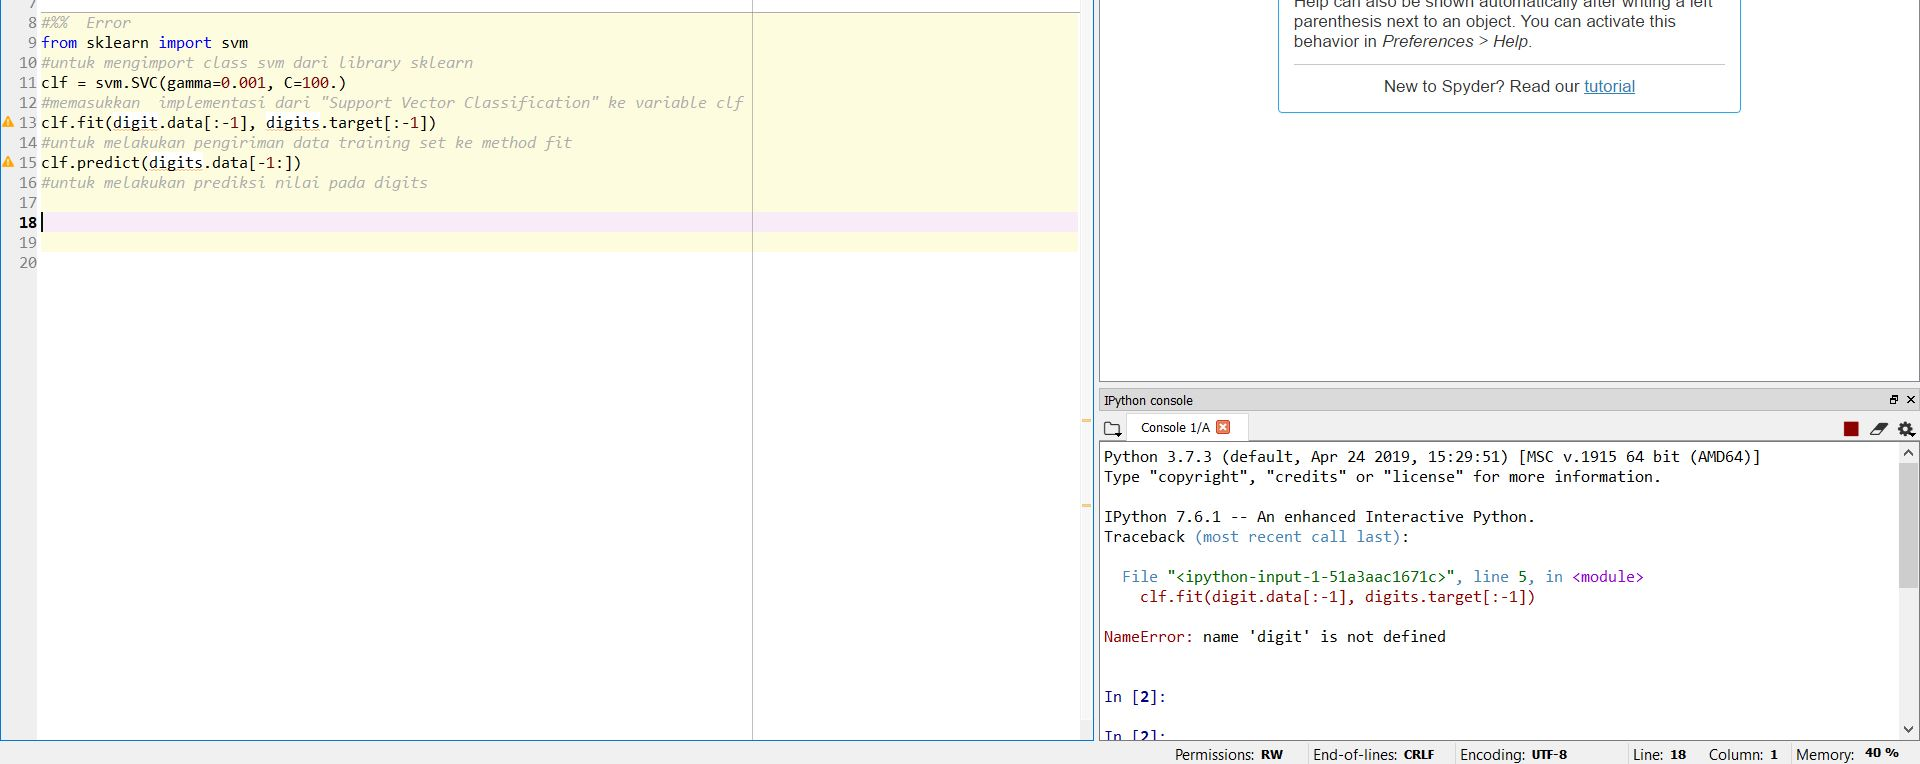
\includegraphics[width=15cm]{figures/1184071/chapter1/3.JPG}
		\centering
		\caption{Name Error}
	\end{figure}
	\newpage\item Tuliskan Kode Error dan Jenis Error
	\hfill\break
	\lstinputlisting[firstline=83, lastline=91]{src/tugas1.py}
\hfill\break
	\item Cara Penangan Error
\hfill\break Tambahkan variabel digits agar kode program dapat terbaca
	\end{enumerate}
	\subsection{Bukti Tidak Plagiarisme}
\begin{figure}[h]
	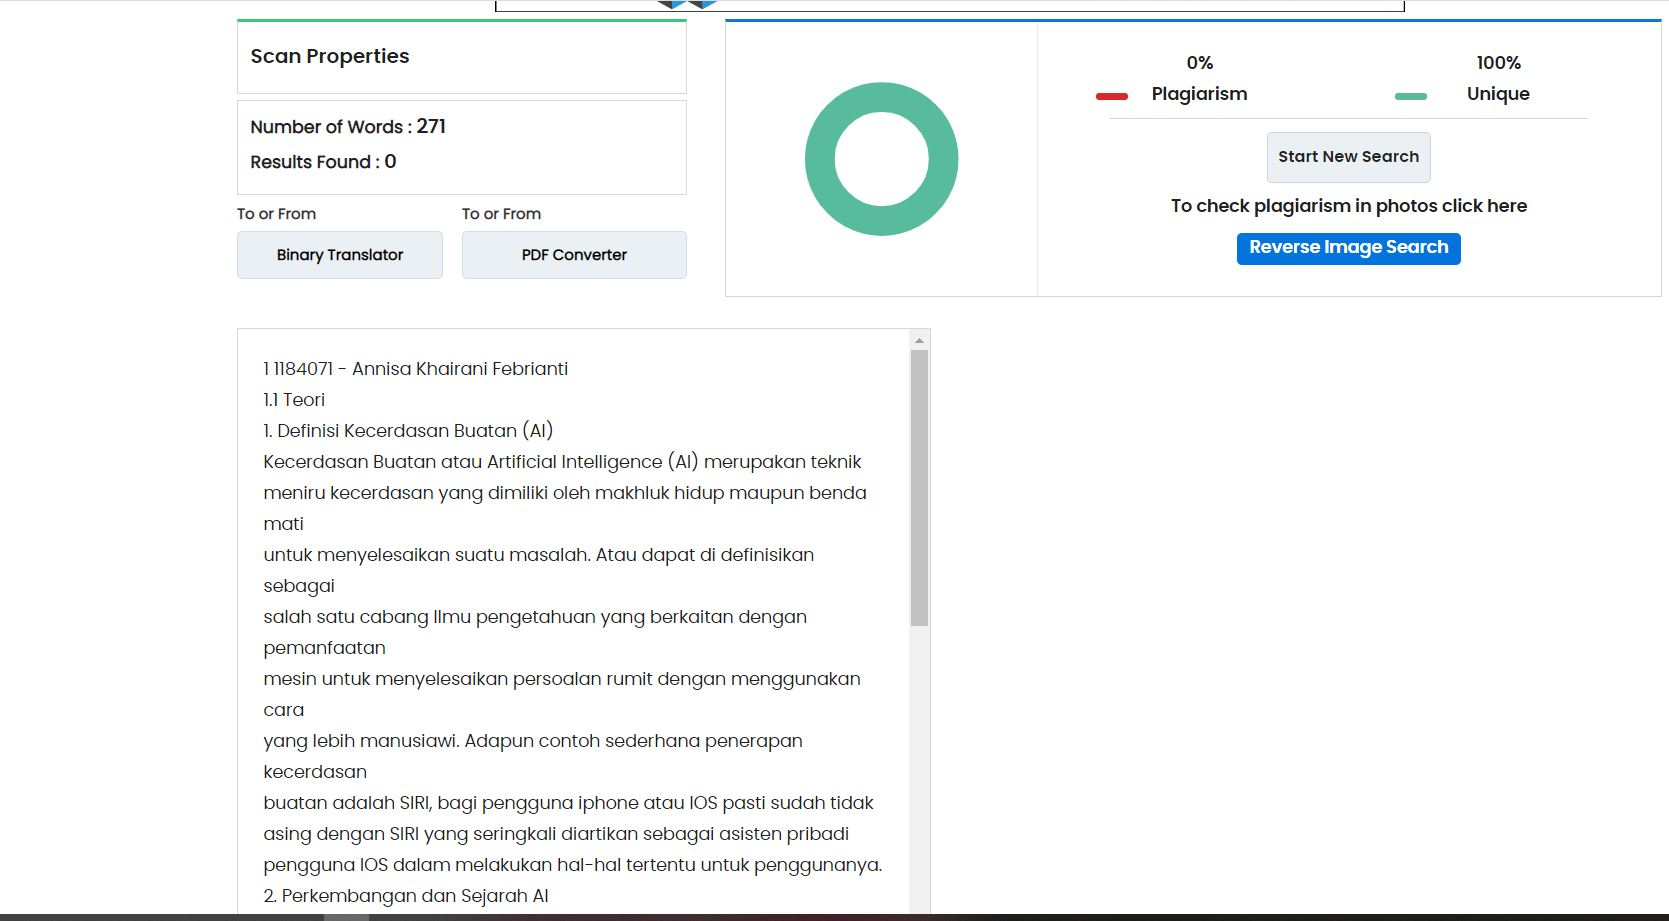
\includegraphics[width=15cm]{figures/1184071/chapter1/4.JPG}
	\centering
	\caption{Bukti Tidak Melakukan Plagiarisme Chapter 1}
\end{figure}



\bibliographystyle{IEEEtran} 
%\def\bibfont{\normalsize}
\bibliography{references}


%%%%%%%%%%%%%%%
%%  The default LaTeX Index
%%  Don't need to add any commands before \begin{document}
\printindex

%%%% Making an index
%% 
%% 1. Make index entries, don't leave any spaces so that they
%% will be sorted correctly.
%% 
%% \index{term}
%% \index{term!subterm}
%% \index{term!subterm!subsubterm}
%% 
%% 2. Run LaTeX several times to produce <filename>.idx
%% 
%% 3. On command line, type  makeindx <filename> which
%% will produce <filename>.ind 
%% 
%% 4. Type \printindex to make the index appear in your book.
%% 
%% 5. If you would like to edit <filename>.ind 
%% you may do so. See docs.pdf for more information.
%% 
%%%%%%%%%%%%%%%%%%%%%%%%%%%%%%

%%%%%%%%%%%%%% Making Multiple Indices %%%%%%%%%%%%%%%%
%% 1. 
%% \usepackage{multind}
%% \makeindex{book}
%% \makeindex{authors}
%% \begin{document}
%% 
%% 2.
%% % add index terms to your book, ie,
%% \index{book}{A term to go to the topic index}
%% \index{authors}{Put this author in the author index}
%% 
%% \index{book}{Cows}
%% \index{book}{Cows!Jersey}
%% \index{book}{Cows!Jersey!Brown}
%% 
%% \index{author}{Douglas Adams}
%% \index{author}{Boethius}
%% \index{author}{Mark Twain}
%% 
%% 3. On command line type 
%% makeindex topic 
%% makeindex authors
%% 
%% 4.
%% this is a Wiley command to make the indices print:
%% \multiprintindex{book}{Topic index}
%% \multiprintindex{authors}{Author index}

\end{document}

